% ============================================================================
%  Chapter 2 -- Literature Review
% ----------------------------------------------------------------------------
%  FORMAT CONVERSION of thesis_writing/chapter_2/chapter_2_full_v2.md
%  (accepted working draft; passed code-truth, coherence, literature and
%  novelty audits). Scientific prose is preserved verbatim; only changes
%  required for valid LaTeX have been made (special-character escaping,
%  en/em dashes, inline math, quotation marks, citation commands,
%  cross-references).
%
%  Source assembly note (editorial metadata, not chapter prose):
%    Assembled draft (v2). Supersedes v1 after the final coherence +
%    code-truth audit (see chapter_2_truth_coherence_audit.md); six minor
%    edits applied -- FactorOrth reference wording, FactorOrth naming,
%    self-distillation wording, a 2.8->2.9 bridge, a de-duplicated sentence
%    in 2.9, and a P27 online-CIL qualifier. Citations are temporary
%    author-year tags in the source; here they resolve to biblatex keys
%    that map to thesis_agent/literature/literature_registry.jsonl.
%
%  CITATION SYSTEM: biblatex, backend=biber, configured in DEIthesis.cls.
%    UPDATED (final Ch.2 revision pass): the class now sets
%    style=numeric-comp (see DEIthesis.cls, "style=authoryear to
%    style=numeric-comp" note), so \parencite/\textcite both render as
%    numeric, comma-compressed bracketed citations (e.g. "[12]"), not the
%    author-year form this note originally described. The in-text commands
%    themselves are unchanged; only their rendered form differs from the
%    original assembly note below.
%    L2P (wang2022learning) and DualPrompt (wang2022dualprompt) are both
%    Wang et al. 2022; the source's generic "(Wang et al., 2022)" for
%    prompt-/prefix-tuning (Sections 2.3 and 2.4) is mapped to
%    wang2022learning (L2P), the canonical "learn to prompt for continual
%    learning" reference.
%
%  FORWARD REFERENCES: resolved. The source's literal "Chapter N" references
%    now use \ref{} against the chapter labels defined in the DEI template
%    (ch:methodology, ch:experimental-setup, ch:results, ch:discussion-conclusion).
%
%  EDITORIAL FIX (2026-09-06 LaTeX integration pass, Chapter 2/3 forward-
%    reference known issue): Section 2.4 previously said the adapter's
%    rank/scaling/target-modules were "specified in Chapter 4." Chapter 3
%    (now converted from chapter_3_full_v2.md, see chapters/chapter_3.tex)
%    is where these quantities are actually DEFINED (Section 3.2); Chapter 4
%    still holds the full experimental configuration. The sentence now
%    distinguishes the two: "defined in Chapter~\ref{ch:methodology}" /
%    "concrete experimental configuration ... in Chapter~\ref{ch:experimental-setup}."
%    No other wording in Chapter 2 was touched.
%
%  EQUATIONS: none as of the final Ch.2 revision pass. The forgetting-measure
%    display equation (former label eq:forgetting) was removed from this
%    chapter -- Section 2.10 now gives only the conceptual BWT/forgetting
%    distinction in prose and defers the exact formula to Chapter 3, which
%    still states it in full under its own label, eq:ch3-forgetting.
%
%  VISUALS (2026-09-06 pass; figure redrawn and one table removed in the
%    final Ch.2 revision pass): see chapter_2/chapter_2_visual_source_options.md
%    for external figures considered and NOT embedded, and
%    thesis_latex/ch2_ch3_latex_integration_audit.md for the original
%    candidate list and rationale.
%    fig:ch2-cl-taxonomy   -- original TikZ taxonomy tree (Section 2.1/2.5)
%    fig:ch2-lora-diagram  -- original TikZ LoRA schematic (Section 2.4),
%                             redrawn in the final revision pass into an
%                             explicit two-panel (training-time branch /
%                             merged inference form) layout; still an
%                             original diagram, not a reproduction of any
%                             external artwork (see the figure's own caption
%                             for provenance).
%    tab:ch2-eval-terminology -- terminology-mapping table (Section 2.9.2)
%    tab:ch2-related-work  -- REMOVED in the final Ch.2 revision pass (was:
%                             synthesis table before the positioning
%                             section). It duplicated the prose positioning
%                             already given in Section 2.11 and was judged
%                             too dense to earn its place; the prose
%                             positioning is preserved in full.
% ============================================================================

\chapter{Literature Review}
\label{ch:literature}

\section{Continual Learning: The Stability--Plasticity Problem}
\label{sec:continual-learning}

Continual learning, also referred to as lifelong or incremental learning,
concerns the training of a single model on a non-stationary stream of data,
in which tasks or groups of classes arrive in sequence and the learner
cannot revisit all of the earlier data \parencite{delange2022continual}. This
departs from the conventional supervised paradigm, where the entire
training distribution is available simultaneously and can be sampled
independently and identically throughout optimisation. Once that assumption
is removed, gradient-based training on newly arriving data tends to
overwrite the parameters responsible for previously acquired competence, a
failure mode known as catastrophic forgetting \parencite{kirkpatrick2017overcoming}.
Because the layers of a neural network are shared across every task,
updates that reduce the loss on the current data distribution can move
parameters away from regions that were favourable for earlier
distributions; forgetting is therefore most naturally understood as
interference in a shared parameter space rather than as the explicit
deletion of stored knowledge \parencite{kirkpatrick2017overcoming,delange2022continual}.

This interference exposes a fundamental tension. A model that is too rigid
retains earlier knowledge but cannot accommodate new classes or domains,
whereas a model that adapts without restraint acquires new competence at
the expense of the old. The continual-learning literature frames this as
the stability--plasticity trade-off: stability is the preservation of
previously learned representations, and plasticity is the capacity to
integrate new information \parencite{delange2022continual}. An effective continual
learner must reconcile the two, and most continual-learning methods can be
read as particular strategies for controlling where, over the course of
training, a model sits on this spectrum.

Continual-learning problems are commonly organised into scenarios that
differ in what changes between successive steps and in what information is
available at inference \parencite{masana2020classincremental,delange2022continual}. In
task-incremental learning, a task identifier is supplied at test time, so
the model need only discriminate among the classes belonging to the
identified task. In domain-incremental learning, the label space is fixed
while the input distribution shifts across steps. In class-incremental
learning (CIL), each step introduces a disjoint set of new classes, the
label space grows cumulatively, and no task identifier is available at
inference, so the model must discriminate among all classes encountered so
far. Class-incremental learning is generally regarded as the most demanding
of the three, because earlier classes must both be retained and placed in
direct competition with later ones under a single decision rule \parencite{masana2020classincremental}.
The present thesis operates entirely within the
class-incremental scenario; the benchmark conventions and protocol choices
that this entails are examined in Section~\ref{sec:cil}, and the remaining scenarios
are not pursued further.

Methods for mitigating forgetting in this setting are usually grouped into
three broad families \parencite{delange2022continual}. Replay-based, or
rehearsal-based, methods retain a subset of past examples, or synthesise
surrogates for them, and interleave these with current data so that earlier
distributions remain represented in the training signal. Regularisation-based
methods add a penalty that discourages changes to the parameters or outputs
deemed important for previous tasks, while storing no past data; Elastic
Weight Consolidation, which penalises movement of parameters identified as
important for earlier tasks, is the canonical instance \parencite{kirkpatrick2017overcoming}.
Parameter-isolation, or architecture-based, methods allocate
distinct parameter subsets to different tasks so that earlier capacity is
shielded from being overwritten by later updates. These families are not
mutually exclusive, and many methods combine elements of more than one. The
work in this thesis adopts a rehearsal-free constraint, meaning that no
past examples are retained in any form; the motivation for this constraint,
and a finer taxonomy of rehearsal-free techniques, are developed in Section~\ref{sec:rehearsal-free}.

Forgetting is not only a phenomenon to be mitigated but also a quantity to
be measured. Backward transfer (BWT) captures the average change in a
task's accuracy between the point at which it was first learned and the end
of training, so that negative backward transfer indicates forgetting
\parencite{lopezpaz2017gradient}. Related forgetting measures summarise, for
each earlier task, the gap between its best recorded performance and its
performance at the end of the sequence \parencite{chaudhry2018riemannian}. Such
measures also make explicit the complementary risk of excessive stability,
sometimes termed intransigence: a model that never updates does not forget,
but neither does it learn \parencite{chaudhry2018riemannian}. The precise definitions
adopted in this thesis, together with their relationship to raw accuracy on
the cumulative label space, are set out in Section~\ref{sec:cl-metrics}.

A final consideration, developed in Section~\ref{sec:recency-bias}, is that the accuracy a
class-incremental model reports on its earlier classes depends not only on
the quality of its internal representations but also on how the evaluation
is conducted. Whether a measured decline in earlier-class accuracy should
be read directly as representational forgetting is therefore an open
question at this stage, and one to which the discussion returns once
evaluation protocols have been introduced. The next section narrows the
focus from continual learning in general to the class-incremental setting
that all of the experiments in this thesis inhabit, and to the benchmark
conventions used to study it.

\section{Class-Incremental Learning: Setting and Benchmark Design}
\label{sec:cil}

Of the continual-learning scenarios distinguished in Section~\ref{sec:continual-learning}, this
thesis is concerned exclusively with class-incremental learning. In CIL, a
model is trained over a sequence of steps, and each step contributes a set
of classes that were not present in any earlier step. The classes
introduced at different steps are disjoint, and the set of categories the
model is expected to recognise grows cumulatively as steps accumulate, so
that after the final step the model must classify inputs across the union
of all classes seen so far \parencite{masana2020classincremental}. The literature also
refers to each such increment as a \enquote{task}; because CIL provides no separate
task structure at inference, this thesis uses the term \enquote{step} consistently
for an incremental class group and reserves no independent role for a task
identity.

The property that most sharply separates CIL from task-incremental learning
is what is available at test time. In task-incremental learning a task
identifier accompanies each input, so the model only has to discriminate
among the classes belonging to the identified task. CIL withholds this
identifier: predictions are made over the entire accumulated label space
through a single classification head, a regime commonly described as
single-head or global evaluation \parencite{masana2020classincremental,delange2022continual}. This
assumption makes the problem substantially harder, and increasingly so as
learning proceeds, because the model must not only represent each class but
also arbitrate between classes that were learned at different times, on
different data, and never jointly, under one decision rule. Each additional
step enlarges the pool of mutually competing categories.

It is in this arbitration that the catastrophic forgetting described in
Section~\ref{sec:continual-learning} becomes most visible. How much earlier information is available
while a step is trained depends on the method: some class-incremental
methods, iCaRL among them, reintroduce a stored subset of earlier examples,
whereas under a rehearsal-free constraint---the regime adopted in this
thesis---each step is trained on its new-class data alone, with no direct
signal preserving the earlier classes, so that the pressure on the shared
representation is correspondingly greater. In systems that classify through
a learned single-head linear layer, a well-documented symptom is that the
classifier becomes biased toward the classes added most recently,
predicting them disproportionately at inference \parencite{masana2020classincremental}; this
reflects that common design rather than a defining property of every
class-incremental method. The mechanisms underlying this bias, and the
techniques proposed to counter it, are examined in Section~\ref{sec:recency-bias}; for present
purposes it is enough to observe that single-head, classifier-based CIL is
particularly exposed to it.

Early class-incremental methods established both a set of algorithmic ideas
and a set of evaluation practices that remain influential. iCaRL \parencite{rebuffi2017icarl} is
representative: it retains a small set of stored examples from earlier
classes, adds a distillation term that encourages the updated model to
preserve its predecessor's responses on those classes, and classifies by
nearest mean of the stored exemplars in feature space rather than through a
learned linear layer. Later work kept the incremental framing while
revisiting each of these ingredients independently. Whether earlier
examples need to be stored at all is the question taken up in Section~\ref{sec:rehearsal-free}.

Empirical study of CIL depends on constructed protocols. A base
classification dataset is partitioned into groups of classes that are
presented in sequence, conventionally under a class ordering that is
randomised but then held fixed, so that reported results do not depend on a
favourable arrangement \parencite{rebuffi2017icarl,masana2020classincremental}.
Protocols differ along several axes: the total number of classes, the
number of incremental steps, whether the first step is larger than the
rest---for instance a substantial initial block followed by smaller
increments---and the number of classes introduced per step. Across the
literature the number of steps ranges from a handful to several dozen
\parencite{masana2020classincremental}. Because the outcome can depend on which classes
happen to arrive early, protocols are frequently evaluated over several
class orderings and the results averaged \parencite{masana2020classincremental}. Performance
is typically summarised in two complementary ways: by the accuracy over the
full accumulated label space measured after each step and averaged across
the sequence, often termed average incremental accuracy, and by the
accuracy after the final step \parencite{masana2020classincremental}. Retention specifically
is read from how the accuracy on an earlier step's classes evolves as later
steps are added; the formal measures used for this purpose are set out in
Section~\ref{sec:cl-metrics}. Image-classification datasets such as CIFAR-100 and subsets
of ImageNet are the usual testbeds.

One axis of protocol design deserves separate attention. For a fixed total
number of classes, the same class space can be divided into a few large
steps or into many small ones. This granularity---referred to here as
protocol depth---is not merely a matter of bookkeeping, because it governs
how many times the model is updated over the course of training and how
much new information each update introduces, both of which plausibly bear
on how much is forgotten. The literature on whether protocol depth has a systematic effect on
forgetting is reviewed in Section~\ref{sec:protocol-depth}. The concrete protocol used in
this thesis, together with the dataset, the class ordering, and the
training configuration, are specified in Chapter~\ref{ch:experimental-setup}. The remainder of
Chapter~\ref{ch:literature} turns to the strategies that have been proposed for limiting
forgetting under the conditions set out above, beginning in Section~\ref{sec:rehearsal-free}
with those that operate without storing any past data.

\subsection{Protocol Depth and Task Granularity}
\label{sec:protocol-depth}

The way a benchmark's class space is divided into incremental steps is not
a neutral formatting decision but an experimental factor in its own right.
Surveys of the area report a broadly consistent pattern: for a fixed
dataset, dividing it into more, and therefore smaller, increments tends to
lower final accuracy and increase measured forgetting \parencite{masana2020classincremental,delange2022continual}.
Plausible explanations include the larger number of sequential updates,
each fitted to a narrower slice of the label space, and the fewer occasions
on which different classes are seen together; which of these dominates is
not settled, and the classifier-competition component is taken up in
Section~\ref{sec:recency-bias}.

Protocol depth, as the term introduced in Section~\ref{sec:cil} is used
here, refers to the number of incremental steps into which a fixed total
class space is partitioned; a controlled protocol-depth comparison would
hold the total class count and the final adaptation capacity fixed while
varying the partition depth. This is narrower than task granularity in the
general sense, which also covers how semantically coarse or fine the
categories themselves are, and distinct again from curriculum or
class-ordering effects, which concern the sequence in which classes are
presented and can matter even when depth is held fixed.

Comparatively little prior work isolates depth through a controlled
design. A recent study \cite{alyamac2026evaluating} asks whether task
granularity affects catastrophic forgetting, but does so by comparing
semantic curriculum orderings---coarse-to-fine, fine-to-coarse, and
flat---over a small subset of classes with a single regulariser (EWC), so
granularity and ordering vary together and the number of steps is not
isolated as an independent variable. A comparison that varies step count
alone, with a fixed method and matched capacity, is less directly
examined, particularly for capacity-growing adapter architectures of the
kind introduced in Section~\ref{sec:lora-cl}.

Protocol depth is not a research question of this thesis. All main
results use the single primary five-step protocol ($5\times20$,
Chapter~\ref{ch:experimental-setup}); only one secondary $4\times25$
diagnostic is reported (Section~\ref{sec:ch5-ablation}), which is not
sufficient to characterise protocol-depth effects systematically. Protocol
depth therefore bounds how far the results reported here can be
generalised, and a controlled protocol-depth study is identified as future
work in Section~\ref{sec:ch6-future-work}.

\section{Rehearsal-Free Continual Learning}
\label{sec:rehearsal-free}

The most direct defence against forgetting is to keep some of the earlier
data. Replay, or rehearsal, stores a subset of past examples---or trains a
generator to produce surrogates---and mixes them into each new step's
training, so that the earlier distributions continue to shape the loss.
Across the continual-learning benchmarks surveyed by \cite{delange2022continual},
replay-based methods are among the most effective, and the
canonical class-incremental method iCaRL \parencite{rebuffi2017icarl}, discussed
in Section~\ref{sec:cil}, depends on a stored exemplar set. Retaining raw training
examples, however, has costs: it consumes a memory budget that grows with
the number of classes, and in many settings the earlier data cannot
lawfully or practically be kept. These considerations motivate
rehearsal-free, or exemplar-free, continual learning, in which raw examples
from previous steps are not retained for later training. This should not be
conflated with a fully memory-free setting, since a rehearsal-free learner
may still preserve model parameters, previous checkpoints, or compact
auxiliary statistics. This thesis adopts the rehearsal-free constraint
throughout.

Rehearsal-free methods are commonly grouped into a small number of
families, most of them refinements of the mitigation categories introduced
in Section~\ref{sec:continual-learning}. Regularisation-based methods add a penalty that discourages
changes to weights or outputs important for earlier steps; Elastic Weight
Consolidation \parencite{kirkpatrick2017overcoming} is the standard reference point.
Parameter-isolation, or architecture-based, methods give different steps
their own parameters, so that earlier capacity is structurally protected
rather than merely regularised. Distillation-based methods constrain the
updated model's outputs to remain close to those of a frozen copy of its
earlier self; Learning without Forgetting \parencite{li2016learning} is the
canonical example, and this mechanism is examined in Section~\ref{sec:kd}. A fourth
line of work leaves the representation untouched and instead re-balances the
final classifier after training to counteract its skew toward recent
classes, which is taken up in Section~\ref{sec:recency-bias}. The families are not exclusive,
and competitive systems usually combine several. Removing the memory buffer
generally costs some accuracy relative to replay-based methods \parencite{delange2022continual};
rehearsal-free research is in large part concerned with
narrowing that gap by making better use of the frozen representation and by
constraining more tightly what each step is permitted to change.

Much recent rehearsal-free work for class-incremental learning has
converged on a common template: a large pretrained model is frozen, and
only a small set of additional parameters is trained per step---whether
input-space prompts \parencite{wang2022learning} or low-rank weight updates
\parencite{wang2023orthogonal,liang2024inflora}. This
keeps the pretrained representation intact, bounds the trainable-parameter
budget, and removes any need to store data from earlier steps. The
adaptation mechanism used in this thesis follows the same template; it is
introduced in Section~\ref{sec:peft-lora}, and its use specifically for continual learning---%
including the design space of approaches that grow, merge, or route such
modules across steps---is the subject of Section~\ref{sec:lora-cl}.

\section{Parameter-Efficient Fine-Tuning and Low-Rank Adaptation}
\label{sec:peft-lora}

Adapting a large pretrained model by fine-tuning all of its weights is
expensive in computation and storage, and in a continual setting it has a
further drawback: every update moves the entire shared representation,
which is precisely what needs to be protected. Parameter-efficient
fine-tuning (PEFT) avoids this by freezing the pretrained weights and
training only a small number of additional or reparameterised parameters
\parencite{houlsby2019parameter}. Several PEFT families exist: bottleneck adapters
insert small trainable modules between the frozen layers \parencite{houlsby2019parameter};
prompt- and prefix-tuning prepend learnable vectors to the input or
to intermediate activations \parencite{wang2022learning}; and low-rank adaptation
modifies the existing weight matrices through an additive low-rank term
\parencite{hu2021lora}. This thesis uses low-rank adaptation exclusively; no
other PEFT family was implemented or compared, which is a deliberate
scoping decision rather than an empirical ranking.

Low-rank adaptation (LoRA) rests on the observation that the weight change
induced by adapting a model to a new task tends to have low effective rank
\parencite{hu2021lora}. For a frozen weight matrix, LoRA keeps that matrix fixed
and learns an update expressed as the product of two thin matrices whose
shared inner dimension---the rank---is far smaller than the dimensions of
the original weight; a scalar factor rescales the update's contribution.
The number of trainable parameters is therefore a small fraction of the
full matrix. Because the learned low-rank update has the same shape as the
original weight matrix, standard LoRA updates can be merged into the base
weights after training, avoiding a separate adapter branch at inference;
unlike inserted adapters, this adds no extra layers. Continual-learning
architectures built on LoRA differ, however, in how far they retain this
property. In transformer models the update is usually applied to the
projection matrices of the attention mechanism, which is also the choice
made here. Figure~\ref{fig:ch2-lora-diagram} summarises this mechanism
schematically.

\begin{figure}[htbp]
\centering
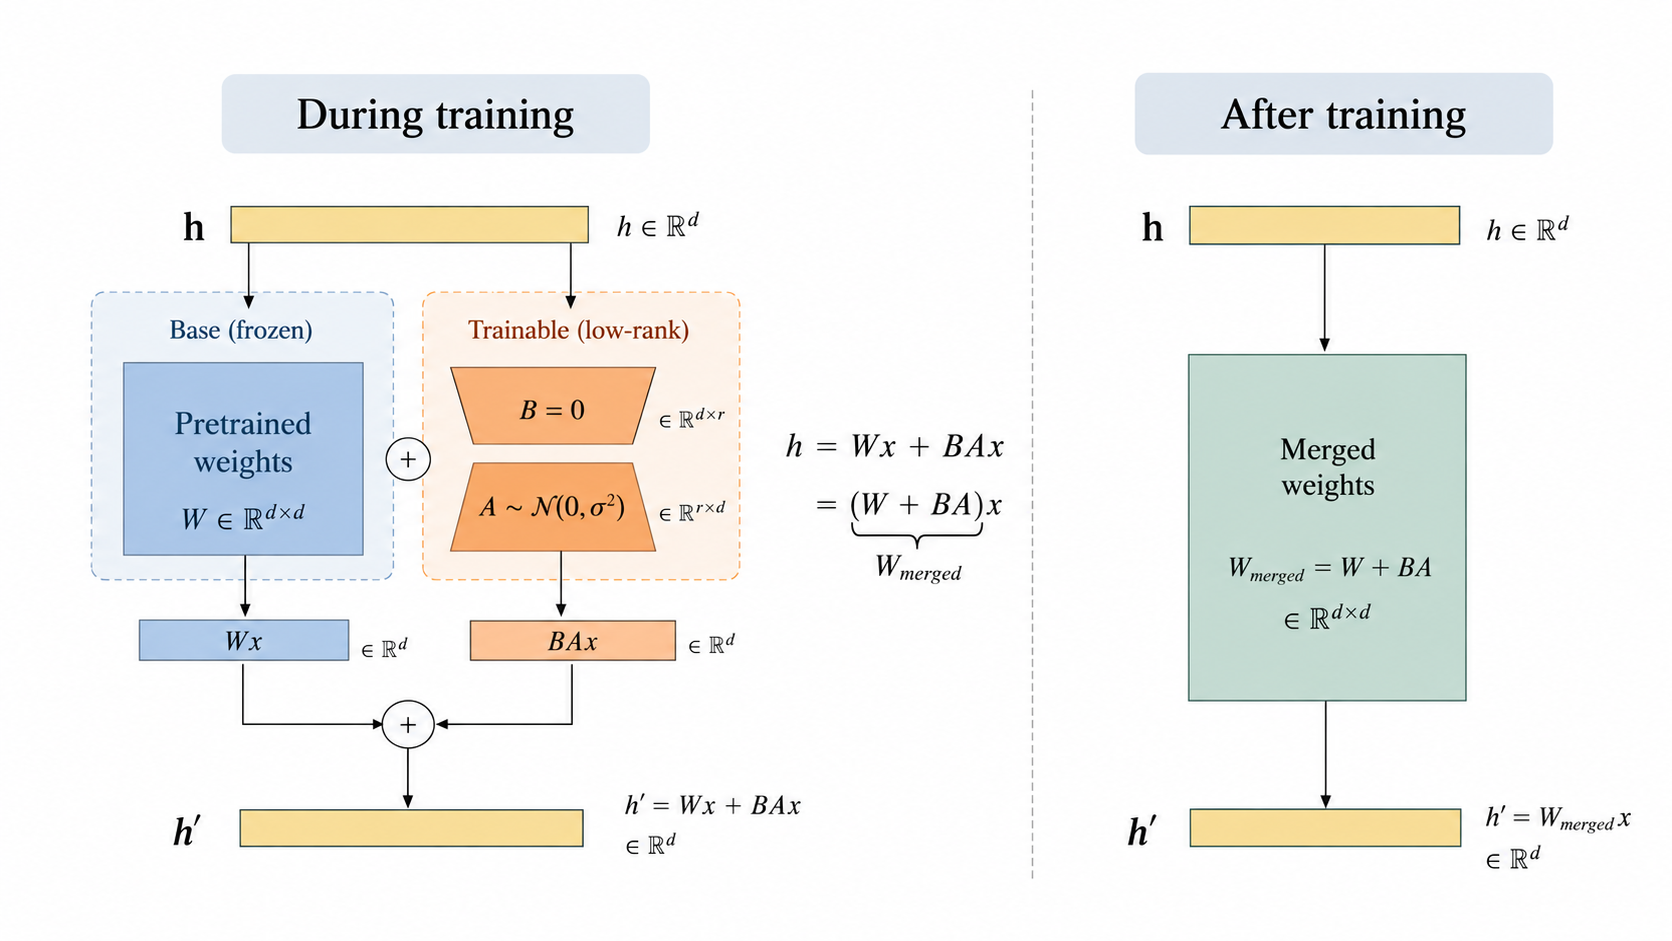
\includegraphics[width=0.85\textwidth]{figures/lora_training_inference_schematic.png}
\caption[Low-rank adaptation (LoRA) schematic]{Schematic illustration of
LoRA during training and after weight merging. During training, the
pretrained weight matrix $W$ remains frozen while the low-rank factors $A$
and $B$ learn the additive update $BA$. After training, the update is
merged into the base matrix as $W_{\mathrm{merged}} = W + BA$, so inference
uses a single weight matrix without a separate LoRA branch. Conceptual
redrawing based on \textcite{hu2021lora}.}
\label{fig:ch2-lora-diagram}
\end{figure}

The pretrained model to which these adapters are attached is the vision
encoder of CLIP \parencite{radford2021learning}, a Vision Transformer \parencite{dosovitskiy2021image}.
CLIP is trained on a large collection of image--text pairs
and produces visual features that transfer well across recognition tasks,
which makes it a strong frozen starting point; its text encoder plays no
role in this thesis, and classification is performed by a trained linear
layer rather than by matching against text prompts. As with the choice of
PEFT family, no alternative backbone was evaluated, and this
single-backbone scope should be borne in mind when interpreting later
results. Refinements of LoRA that quantise the frozen weights, decompose
the update differently, or allocate rank adaptively have since been
proposed; none is used here. The adapter---its rank, its scaling, and the
modules it is applied to---is defined in Chapter~\ref{ch:methodology}, and its
concrete experimental configuration is specified in Chapter~\ref{ch:experimental-setup}.
How low-rank adaptation is used as the vehicle for continual
learning, rather than for one-off task adaptation, is the subject of
Section~\ref{sec:lora-cl}.

\section{Continual Learning with LoRA-Based Adaptation}
\label{sec:lora-cl}

Using low-rank adaptation for a sequence of steps rather than for a single
task confines all adaptation to a small and structurally regular set of
parameters. This makes the composition question explicit---how should the
per-step updates be combined?---and the literature offers three broad
answers.

The first keeps separate per-step parameters and selects or combines them
at inference. The prompt-based methods L2P \parencite{wang2022learning} and
DualPrompt \parencite{wang2022dualprompt} are the prominent instances: they attach a
set of learnable prompt vectors to a frozen backbone and retrieve the
relevant ones for each input through a learned key--query mechanism that
needs no task label at test time, with DualPrompt separating task-shared
from task-specific prompts. These methods operate in input space rather
than weight space and are noted here as a sibling family rather than a
comparison point.

The second strategy trains an adapter independently at each step and merges
the results into a single set of weights afterwards; this is the subject of
Section~\ref{sec:model-merging}.

The third maintains a persistent low-rank component that is extended or
updated as steps arrive. SD-LoRA \parencite{wu2025sdlora} appends a new low-rank
direction pair at each step, freezing the earlier directions while leaving
their magnitudes trainable. CL-LoRA \parencite{he2025cllora} combines a shared
adapter that is updated throughout with per-task adapters that are frozen
after their step, re-running each task's adapter at inference so that its
inference cost grows with the number of steps. InfLoRA \parencite{liang2024inflora}
restricts each step's update to a subspace chosen so as not to interfere
with earlier tasks. Merge-before-Forget \parencite{qiao2025merge}, in the
language domain, consolidates each step into one rank-capped adapter by
merging before the next step begins. The broader literature therefore
establishes persistent, expandable, and selectively composed low-rank
adaptation as an active continual-learning design space, whose members
differ substantially in whether past components are frozen, retained
separately, continuously updated, or merged. It is this design space, not
any single architecture within it, that is well established.

This thesis compares two points in this space: a persistent adapter whose
rank is extended step by step, termed RankExt, and a set of independently
trained per-step adapters combined by simple averaging, termed SimpleAvg;
both are defined in full in Chapter~\ref{ch:methodology}. RankExt belongs to the
growing-adapter family described above and shares its overall shape; its
distinguishing features are at the level of mechanism rather than concept.
The parameters contributed by earlier steps are hard-frozen with no
remaining trainable degrees of freedom, in contrast to SD-LoRA's trainable
magnitudes or CL-LoRA's continuously updated shared component; interference
between old and new parameters can be further limited by a loss term that
penalises their overlap (Section~\ref{sec:orthogonality}) and, optionally, by self-distillation
from an earlier checkpoint of the model (Section~\ref{sec:kd}). Inference
uses a single persistent adapter and requires no per-step routing or
repeated step-specific forward passes; however, the adapter's parameter and
computation footprint grows with its cumulative rank. SimpleAvg,
by contrast, is included as a deliberately simple merging baseline---the
independent-adapter-averaging case, treated in Section~\ref{sec:model-merging}---and is not put
forward as a new method. The purpose of pairing them is the
retention--plasticity comparison that motivates the primary research
question, not the introduction of either as a novel architecture.
Figure~\ref{fig:ch2-cl-taxonomy} places this pair, and the broader
LoRA-based continual-learning design space around them, within the
taxonomy developed over the course of this and the preceding sections.

\begin{figure}[htbp]
\centering
\resizebox{\textwidth}{!}{%
\begin{tikzpicture}[
  every node/.style={font=\small, align=center},
  root/.style={draw, thick, rounded corners, minimum height=0.9cm, minimum width=3.2cm, fill=black!5},
  fam/.style={draw, thick, minimum height=0.9cm, minimum width=3.6cm},
  leaf/.style={draw, minimum height=0.8cm, minimum width=3.6cm},
  edge from parent/.style={draw, -{Latex[length=1.8mm]}},
  level 1/.style={sibling distance=4.1cm, level distance=1.6cm},
  level 2/.style={sibling distance=3.9cm, level distance=1.7cm},
  level 3/.style={sibling distance=3.9cm, level distance=1.7cm},
]
\node[root] {Continual learning\\\footnotesize(Section~\ref{sec:continual-learning})}
  child { node[fam] {Replay-based} }
  child { node[fam] {Regularisation-based\\\footnotesize (e.g.\ EWC)} }
  child { node[fam] {Parameter-isolation /\\architecture-based} }
  child { node[fam] {Pretrained backbone,\\PEFT-based\\\footnotesize(Section~\ref{sec:peft-lora})}
    child { node[leaf] {LoRA-based adaptation\\\footnotesize(Section~\ref{sec:lora-cl})}
      child { node[leaf, minimum width=3.4cm] {Selected/composed\\per-step prompts\\\footnotesize(L2P, DualPrompt)} }
      child { node[leaf, minimum width=3.4cm, fill=black!5] {Independent-per-step,\\merged post-hoc\\\footnotesize(\textbf{SimpleAvg}; Section~\ref{sec:model-merging})} }
      child { node[leaf, minimum width=3.4cm, fill=black!5] {Persistent,\\growing-rank\\\footnotesize(\textbf{RankExt}; SD-LoRA,\\CL-LoRA, InfLoRA)} }
    }
  };
\end{tikzpicture}%
}
\caption[Continual-learning taxonomy]{Taxonomy of continual-learning
strategies as developed in this chapter. The three families on the left are
introduced in Section~\ref{sec:continual-learning}; the rehearsal-free,
pretrained/PEFT-based template (Sections~\ref{sec:rehearsal-free}--\ref{sec:peft-lora})
and the three strategies for organising LoRA parameters across an
incremental sequence (Section~\ref{sec:lora-cl}) are drawn as its own
branch rather than as a fourth sibling of the original three, since it cuts
across them (most concretely, it is a rehearsal-free specialisation of the
regularisation- and parameter-isolation-based families). Shaded leaves mark
the two strategies compared in this thesis. Original synthesis figure; no
single source in the literature presents this exact taxonomy.}
\label{fig:ch2-cl-taxonomy}
\end{figure}

\section{Model Merging}
\label{sec:model-merging}

Model merging combines the weights of several independently trained
networks into a single set of parameters, without further training and
without keeping the individual models at inference. The idea was
popularised by model soups \parencite{wortsman2022model}, which showed that
averaging the weights of models fine-tuned from a shared initialisation
with different hyperparameters can improve accuracy at no inference cost.
Task arithmetic \parencite{ilharco2023editing} generalised the operation: each
fine-tuning run is summarised by a task vector, the difference between the
fine-tuned and the base weights, and these vectors can be added to combine
capabilities or negated to remove them.

The quality of a merge is governed by interference between the
contributions being combined. When two updates disagree about the sign or
magnitude of a change to the same parameter, averaging them partially
cancels both, and the merged model can underperform each of its
constituents. TIES-Merging \parencite{yadav2023ties} is a representative
response: it discards the smallest changes, resolves sign disagreements by
majority, and only then averages the survivors. A family of such
interference-aware schemes now exists, differing in how conflicts are
detected and reconciled.

For continual learning, merging has a clear appeal. Each step can be
trained in complete isolation---with no access to earlier steps and no
interaction with their parameters during optimisation---and the results
folded into one model only afterwards. The corresponding difficulty is that
the merge must reconcile updates that were never optimised together, on
data distributions that do not overlap, which is the regime in which
interference is expected to be most severe. None of the methods above is
itself a continual-learning method: model soups merges models of the same
task, and task arithmetic performs post-hoc capability editing. They
establish the general operation on which a continual merging strategy can
be built.

This thesis includes one such strategy as a baseline, using the simplest
available merge---an unweighted average of the per-step contributions---%
chosen deliberately for its simplicity, so that the later comparison
isolates the effect of the adaptation architecture rather than of merge
sophistication. Its instantiation for low-rank adapters, and its
relationship to published work on merging adapters across sequential tasks,
are the subject of Section~\ref{sec:adapter-merging}.

\subsection{Weight Averaging / Adapter Merging}
\label{sec:adapter-merging}

The merge operation of Section~\ref{sec:model-merging} can be applied to low-rank adapters
rather than to full weight matrices. This can be done in more than one way,
and the ways are not equivalent: one may average the low-rank factors of
each step's update, or first reconstruct each step's dense weight-change
matrix from its factors and then average those dense matrices. This thesis
takes the second route---each step's update is reconstructed as a
full-size weight-change matrix, and the per-step matrices are averaged
elementwise, so the averaging is of dense updates, not of factors.

This interacts with the capacity argument of Section~\ref{sec:lora-cl}. Each per-step
update is confined to a bounded number of directions; the elementwise
average of several such dense updates generally spans more directions than
any one of them, because their column spaces need not coincide. A merged
adaptation can therefore occupy a higher effective rank than a single
step's update---a point of contrast with an architecture whose total rank
is fixed by construction.

Adapter merging tailored to continual learning, and going beyond a plain
average, is an active line of work. GLAM, previously HAM \parencite{testa2025glam},
groups per-task adapters by similarity and then prunes, rescales,
and importance-weights them within each group before merging.
Merge-before-Forget \parencite{qiao2025merge}, in the language domain and
already noted in Section~\ref{sec:lora-cl}, folds each step into one persistent adapter
sequentially, using a recency-weighted combination and an orthogonal
initialisation for each new step.

A separate line of work asks whether merging strategies developed for fully
fine-tuned task vectors---including the interference-aware schemes of
Section~\ref{sec:model-merging}---transfer cleanly to LoRA modules in the
first place. Decouple and Orthogonalize (DO-Merging) \parencite{zheng2025domerging} reports that applying
such full-fine-tuning-oriented merging methods directly to LoRA adapters can
degrade performance, and identifies large magnitude variation across the
LoRA modules being combined as one contributor: a module whose update has a
small overall magnitude can be dominated during elementwise averaging even
when its direction is informative. Its proposed remedy decouples each
update into a magnitude and a direction component, merges the two
separately, and applies a data-free, layer-wise orthogonality constraint
when combining the directional components to reduce this interference. This
is noted here as motivation for treating the merge step itself, not only
the per-step adaptation architecture, as a possible source of degradation;
it is not evidence about the specific baseline adopted below. The
unweighted dense-update average used as this thesis's own merging baseline
performs no magnitude/direction decoupling and applies no orthogonality
constraint at merge time, and should not be read as an instance of, or a
test of, the DO-Merging mechanism.

The merging baseline used in this thesis sits at the opposite, minimal end
of this range: each step's adapter is trained fully independently, and the
per-step dense updates are combined by a single unweighted average taken
once, after the whole sequence, with no clustering, importance weighting,
or orthogonalisation; the per-class classifier rows are copied from the
step that trained them rather than averaged. The general merging literature
suggests that so minimal a scheme should be exposed to the interference
between non-jointly-optimised updates described in Section~\ref{sec:model-merging}; whether that
expectation holds in this setting is examined in Chapter~\ref{ch:results}. The baseline is
included as a controlled comparator for the architectural approach of
Section~\ref{sec:lora-cl}, not as a contribution to merging methodology, and its
simplicity is a deliberate design choice rather than a gap identified in
the literature.

\section{Knowledge Distillation for Continual Learning}
\label{sec:kd}

Knowledge distillation (KD) trains one model to reproduce the
temperature-softened output distribution of another, so that the relative
scores of the non-predicted classes, and not only the top prediction,
carry information \parencite{hinton2015distilling}. It was introduced as a compression
technique, with a small student imitating a larger teacher.

In continual learning the mechanism is re-purposed. The teacher is a frozen
copy of the model as it stood at an earlier point in the sequence, and the
distillation term discourages the current model's outputs, on the inputs it
is now training on, from moving away from what that earlier model would have
produced. Learning without Forgetting \parencite{li2016learning} introduced this
idea for incremental classification: because no earlier data is kept, the
earlier model's responses to the current step's inputs act as a soft record
of what it had learned. Implementations differ in what is matched---the
outputs for previously seen classes only, or the full output distribution---%
and in whether a single shared head or separate per-task heads are
distilled; the original formulation of Learning without Forgetting was
multi-head. In this thesis, both variants appear: within RankExt,
distillation acts on the full output distribution over all classes seen so
far, whereas within SimpleAvg it is restricted to the previously seen
classes. In both families a frozen earlier state of the model serves as
the teacher, and both the teacher construction and the distillation scope
are family-specific, as defined in Chapter~\ref{ch:methodology}. The technique is therefore used here as a
form of self-distillation between successive states of the same model
family, aimed at stabilising continual learning rather than compressing a
larger teacher into a smaller student.

Distillation is frequently paired with rehearsal. Dark Experience Replay
\parencite{buzzega2020dark}, for example, stores output logits from earlier
training in a buffer and distils against them throughout the sequence. The
setting of this thesis is stricter, as established in Section~\ref{sec:rehearsal-free}: no
buffer is available, so a distillation signal can come only from a frozen
snapshot of the model's own earlier training, refreshed as the sequence
advances; how that snapshot is constructed differs between the two families
and is specified in Chapter~\ref{ch:methodology}.

A second anchoring mechanism, used only in some variants, should not be
confused with this distillation: a loss that pulls intermediate features
toward those of the frozen, never-trained backbone introduced in Section~\ref{sec:peft-lora}.
That anchor references the pretrained model rather than a prior
training state; its experimental configuration is specified in
Chapter~\ref{ch:experimental-setup}.

Within the growing-adapter family of Section~\ref{sec:lora-cl}, distillation from an
earlier state is one of two mechanisms whose contribution this thesis
examines; the other, a penalty on the overlap between old and new
parameters, is the subject of Section~\ref{sec:orthogonality}. How the two compare is the
second research question, taken up in Chapter~\ref{ch:results}.

\section{Orthogonality-Based Regularization for Continual Learning}
\label{sec:orthogonality}

A recurring idea for limiting interference is to keep the parameter changes
made for a new step orthogonal to the directions that earlier steps rely
on: if the new update does not project onto the subspace the earlier
solution occupies, it should perturb the earlier behaviour less. This
principle has been applied at two different loci.

The first is gradient or representation space. Orthogonal Gradient Descent
(OGD) \parencite{farajtabar2020orthogonal} stores a basis for the gradients of earlier
tasks and projects each new gradient onto its orthogonal complement before
the update is applied; Gradient Projection Memory (GPM) \parencite{saha2021gradient}
does the same using a basis extracted from the representations of past
tasks. In
both, orthogonality is enforced by a projection during optimisation rather
than by a term in the loss.

The second locus is the parameters themselves, and for low-rank adapters it
has become an active line of work. O-LoRA \parencite{wang2023orthogonal} keeps the
LoRA subspaces of successive tasks close to orthogonal by adding a soft
penalty on the squared overlap between the current task's factors and each
earlier task's, summed over the earlier tasks. BiLoRA \parencite{zhu2025bilora}
reaches a similar end by different means: it reparameterises the adapter
over fixed orthogonal bases, so that near-orthogonality between tasks holds
by construction and no penalty term is needed. These are two mechanism
classes---a soft trained penalty and a structural guarantee---for the same
objective.

Imposing orthogonality among LoRA components does not, by itself, guarantee
that the entries of the underlying pretrained representation that matter
most for earlier steps stay unchanged: orthogonality constrains how the new
and old low-rank factors relate to each other, but says nothing directly
about which entries of the resulting dense weight change are large.
LoRAC \parencite{ling2026lorac} makes this limitation explicit for
orthogonal LoRA composition specifically---it reports that parameters
identified as critical for earlier steps can still change substantially
after later steps are learned even when the LoRA components introducing
those steps are constructed to be mutually orthogonal, and addresses this
by additionally freezing the parameter entries identified as most important
for earlier steps, on top of the orthogonal composition itself. This result
is cited here as a caution against treating parameter-space orthogonality
as a sufficient mechanism for forgetting mitigation on its own; it is not a
claim about the FactorOrth formulation below, which this thesis evaluates
empirically rather than assumes to be complete.

FactorOrth is the thesis-wide name used for orthogonality-based
regularisation---the loss term referred to in Section~\ref{sec:lora-cl}---and
belongs to the soft-penalty class. Its concrete formulation is
family-specific: for SimpleAvg, orthogonality is imposed on reconstructed
dense updates, whereas for RankExt it is imposed directly on the low-rank
factors. In SimpleAvg, the penalty acts on the squared cosine similarity
between the current step's reconstructed dense update and each earlier
step's dense update. In RankExt, it penalises the overlap between the new
block's normalised low-rank factors and the frozen accumulated prior rank
blocks, so the penalty is layered on an architecture whose earlier
parameters are already frozen. The RankExt formulation differs from O-LoRA
in how the penalty is formed---it constrains both factors of the
decomposition against one combined reference rather than against a pool of
per-task matrices kept separately---but in neither family is the
underlying idea, a soft orthogonality penalty between old and new low-rank
updates, introduced here: O-LoRA is a representative prior example of the
soft-penalty form, and BiLoRA represents the stronger, structural
alternative.
The exact formulation, and an assessment of how much the term contributes
on top of distillation, are given in Chapters~\ref{ch:methodology} and~\ref{ch:results} respectively.

Distillation from an earlier state, described in Section~\ref{sec:kd}, and this
orthogonality penalty are the two mechanisms whose roles within the
growing-adapter family the second research question examines.

\section{Recency Bias and Evaluation-Protocol Effects}
\label{sec:recency-bias}

The preceding sections concerned mechanisms for limiting forgetting; this
section and the next turn to how retention is measured, beginning with a
phenomenon that complicates the measurement. Section~\ref{sec:cil} noted that a
class-incremental classifier with a single shared head tends to favour the
classes it has seen most recently. This effect has
a name and a well-documented mechanism. As successive steps train on their
own classes, the classifier's weight rows for the newer classes come to
have larger norms, and their logits are systematically larger, than those
of the older classes; under a single argmax over all classes, the newer
classes therefore win disproportionately. The phenomenon is generally
called task-recency bias \parencite{masana2020classincremental,liang2023new}. The
imbalance is sharpened when earlier data is not replayed, because each step
then sees its own classes only as positive examples and every other class
only as a negative, which drives the newer rows to grow relative to the
older ones. It should not be confused with fairness- or demographic-related
senses of \enquote{bias}: it is a property of the classifier's output scale, not of
the data or of any protected attribute.

The distinction that matters for this thesis is that task-recency bias is a
competition effect at the output layer, and it need not track the quality
of the underlying representation. A model can retain a good internal
representation of an earlier class and still misclassify it, simply because
a more recent class produces a larger score. The phenomenon has been
documented directly, by measuring the weight norms and logit magnitudes of
the older and newer class groups \parencite{liang2023new}.

The literature offers two broad responses. One is to correct the classifier
after training, so that the classes compete on equal terms; this is the
subject of Section~\ref{sec:calibration}. The other is to change how retention is measured,
so that the output-competition effect is separated from genuine
representational change; this is the subject of Section~\ref{sec:open-restricted}. This section
establishes that classifier-scale imbalance is an established source of
task-recency bias and can produce apparent forgetting even when useful
earlier representations remain available; distinguishing this competition
effect from genuine representational degradation motivates the evaluation
analysis developed in Section~\ref{sec:open-restricted}.

\subsection{Classifier Calibration in CIL}
\label{sec:calibration}

One response to task-recency bias is to adjust the trained classifier
directly, leaving the learned representation untouched. Two established
methods define the space. Weight Aligning \parencite{zhao2020maintaining} observes that
the weight rows for newly added classes tend to have larger norms than
those for old classes, and rescales the new-class rows by the ratio of the
average old-class norm to the average new-class norm, applied once after
the final step; the old-class rows are left unchanged, and no held-out data
is required. Bias Correction \parencite{wu2019large} instead learns a
two-parameter linear transformation---a scale and a shift---applied to the
logits of the new classes, fitting those parameters on a small held-out
validation set. The two differ in kind: one is a closed-form norm-matching
rule, the other a learned correction that consumes labelled data. Because
both act only on the output layer, they can rebalance which class wins the
argmax but cannot recover a representation that has genuinely drifted.

The calibration applied in this thesis belongs to the Weight Aligning
family and is used only as a partial remedy discussed alongside the third
research question, not as one of the thesis's contributions. Its basic form
generalises Weight Aligning from a two-group correction---old classes
versus new---to a per-step rescaling in which every step's block of rows,
the earliest included, is moved toward a shared target norm, where Weight
Aligning would have held the oldest rows fixed. A further variant computes
separate targets for groups of steps that were trained under the same
conditions, and a third additionally modulates each step's target by a
signal derived from that step's validation loss. Only the first two stay
close to Weight Aligning's mechanism; the third is related to it in aim but
not in form. The complete procedure should therefore not be described as a
direct implementation of Weight Aligning. Its formulation is given in
Chapter~\ref{ch:methodology}, and the degree to which it narrows the gap it targets is
assessed in Chapter~\ref{ch:discussion-conclusion}.

\subsection{Task-Agnostic vs.\ Task-Oracle Evaluation}
\label{sec:open-restricted}

Accuracy on a class-incremental model can be measured in two ways that
differ only in what the classifier is allowed to choose between. In
task-agnostic evaluation---also called task-free, and corresponding to the
Class-IL accuracy reported in most of the literature---the argmax runs over
every class seen so far, with no task identifier supplied \parencite{masana2020classincremental,delange2022continual}. In task-oracle evaluation---task-aware,
corresponding to Task-IL accuracy---a task identifier is provided at test
time and the argmax is restricted to the classes introduced at that step.
Task-oracle accuracy is normally reported as a diagnostic upper bound
rather than as the headline number, because supplying the task identifier
removes a large part of the problem \parencite{masana2020classincremental}. This thesis
refers to the two modes as open and restricted evaluation respectively.
These two evaluation modes correspond respectively to task-agnostic
(Class-IL) and task-oracle/task-aware evaluation; the correspondence is
conceptual rather than an exact equivalence, since restricted evaluation
here masks the logits of the same single model, whereas Task-IL setups in
the literature may differ in implementation and head organisation. The
terms are used consistently from Chapter~\ref{ch:methodology} onward, and
Table~\ref{tab:ch2-eval-terminology} summarises the correspondence.

\begin{table}[htbp]
\centering
\begin{tabularx}{\textwidth}{@{}>{\raggedright\arraybackslash}p{2.6cm} >{\raggedright\arraybackslash}p{3.1cm} X >{\raggedright\arraybackslash}p{2.4cm}@{}}
\toprule
\textbf{This thesis} & \textbf{Standard term} & \textbf{Argmax is taken over} & \textbf{Role} \\
\midrule
Open evaluation & Task-agnostic / task-free (Class-IL) & every class seen so far; no task identifier supplied & primary, headline metric \\
Restricted evaluation & Task-oracle / task-aware (Task-IL) & only the classes introduced at the queried step; task identifier supplied & diagnostic upper bound \\
\bottomrule
\end{tabularx}
\caption[Open/restricted evaluation terminology]{Terminology used in this
thesis for the two evaluation modes distinguished above, and their
correspondence to the standard terms of \cite{masana2020classincremental}.}
\label{tab:ch2-eval-terminology}
\end{table}

The two modes isolate different things. Restricted evaluation removes
cross-step competition: a class is scored only against the classes it was
learned alongside, so its result reflects how well the model separates that
step's classes and is much less affected by the cross-step output-scale
imbalance described in Section~\ref{sec:recency-bias}. Open evaluation
retains that competition, so the gap between a model's restricted and open
accuracy on the same earlier step provides a diagnostic indication of how
much of its apparent forgetting may be associated with losing the argmax to
more recent classes rather than with a degraded representation of the
earlier ones.

Both evaluation modes are individually standard. What the literature
reviewed here does not identify is their use as a paired diagnostic---%
computing open and restricted accuracy from the same forward pass on the
same model and reading the difference as a diagnostic indication of the
classifier-competition contribution to apparent forgetting, rather than as a
definitive causal decomposition of it. The closest
prior study of task-recency bias, conducted in an online class-incremental
setting, diagnoses the effect by inspecting classifier weights and logits
directly and reports accuracy under a single evaluation mode \parencite{liang2023new}.
This motivates the paired diagnostic adopted in this thesis,
whose construction is given in Chapter~\ref{ch:methodology} and whose results are reported in
Chapter~\ref{ch:results}.

\section{Continual-Learning Evaluation Metrics}
\label{sec:cl-metrics}

Three quantities are used to report retention in this thesis, alongside raw
accuracy. The primary headline metric used in this thesis is final open
accuracy over all classes seen after the complete incremental sequence.
Per-step accuracies are retained to analyse continual trajectories and to
compute backward transfer and forgetting. The class-incremental literature
also commonly reports average incremental accuracy, the mean of all-seen
accuracy across the steps of the sequence
\parencite{masana2020classincremental}; it is a standard metric but not the
headline metric of this thesis. The two measures below summarise how
accuracy on earlier steps changes over the sequence.

Backward transfer \parencite{lopezpaz2017gradient} compares a step's final
performance with its performance when it was first learned, whereas the
forgetting measure \parencite{chaudhry2018riemannian} compares final
performance with the best performance previously attained for that step.
These measures capture related but distinct aspects of retention: backward
transfer is anchored to a single reference point (accuracy immediately after
a step was first learned), whereas forgetting is anchored to whichever later
point gave that step its best recorded accuracy. The exact definitions, and
the implementation-specific treatment adopted in this thesis, are given in
Chapter~\ref{ch:methodology}.

Forward transfer---the influence of earlier steps on a step not yet
trained---is defined in the same literature but is not reported as a result
of this thesis, because the corresponding project output was not validated
for reliable interpretation; the term is mentioned here only to complete the
standard metric vocabulary. Restricted accuracy, used together with open
accuracy as the diagnostic of Section~\ref{sec:open-restricted}, is defined
there.

\section{Positioning of This Thesis Relative to Prior Work}
\label{sec:thesis-positioning}

The preceding sections place this thesis at the intersection of
rehearsal-free class-incremental learning (Section~\ref{sec:rehearsal-free}) and low-rank
adaptation of a frozen backbone (Sections~\ref{sec:peft-lora} and~\ref{sec:lora-cl}). The thesis does not
introduce this intersection; it is an established and active setting. Its
work is to compare two strategies for adapting a LoRA-based model across
steps, to examine the mechanisms that stabilise one of them, and to sharpen
how retention is measured. The paragraphs that follow read research
question by research question, stating where each part sits relative to the
prior work reviewed above and which specific gap it addresses.

\textbf{The two adaptation strategies (RQ1, Contribution 1).} The persistent, growing-rank
adapter studied in this thesis---RankExt---belongs to the design space of
single-adapter, growing-capacity LoRA methods for continual learning
described in Section~\ref{sec:lora-cl}. That design space is well populated: SD-LoRA \parencite{wu2025sdlora}
is very close at the level of architectural framing, and
CL-LoRA \parencite{he2025cllora} and Merge-before-Forget \parencite{qiao2025merge}
overlap in part. The thesis therefore does not claim to introduce
growing-rank LoRA for continual learning. What distinguishes RankExt within
that space is its mechanism: the parameters from earlier steps are
hard-frozen with no remaining trainable degrees of freedom, new capacity is
added by concatenating rank rather than by re-scaling existing directions,
and it can be combined with distillation and an orthogonality penalty on a
frozen vision backbone. The other strategy---SimpleAvg---is a deliberately
simple merging baseline: independent per-step adapters combined by an
unweighted average of their dense updates (Section~\ref{sec:adapter-merging}). It is not
offered as a new method; its role is to give the persistent-adapter
approach a controlled point of comparison. The two families are not
perfectly matched in effective capacity, which Chapter~\ref{ch:methodology} treats as a stated
scope condition on RQ1 rather than a confound to be removed.

\textbf{The two stabilising mechanisms (RQ2, Contribution 2).} Distillation from
an earlier state of the model, used in the RankExt family, descends from
Learning without Forgetting \parencite{li2016learning} and is not novel. The
orthogonality penalty, FactorOrth, belongs to the established family of
soft orthogonality regularisers for LoRA-based continual learning; O-LoRA
\parencite{wang2023orthogonal} is a representative prior example of the
soft-penalty form and BiLoRA \parencite{zhu2025bilora} of the structural
alternative. The thesis does not claim the
orthogonality idea. Its contribution here is the systematic ablation of
this particular formulation and its integration within RankExt, including
how it interacts with distillation.

\textbf{The evaluation lens (RQ3, Contribution 3).} Task-recency bias, and the
classifier-scale mechanism behind it, are well established \parencite{zhao2020maintaining,wu2019large,liang2023new}, and the distinction between
task-agnostic and task-oracle evaluation is standard. The paired use of the
two evaluation modes---reading the gap between open and restricted accuracy
on the same forward pass as a diagnostic indication of the
classifier-competition contribution to apparent forgetting, rather than as a
definitive causal decomposition of it---is not identified in the literature
reviewed here; the closest prior study of task-recency bias \parencite{liang2023new}
diagnoses the effect differently and reports a single evaluation
mode. This paired diagnostic is the distinctive element. The post-hoc
classifier calibration the thesis also applies is a generalisation of
Weight Aligning \parencite{zhao2020maintaining} and is treated as a partial remedy, not
as a contribution.



Taken together, the contribution of this thesis is comparative, ablative,
and diagnostic rather than the introduction of a new architecture or
regulariser. Each research question addresses a specific gap left by the
work reviewed above: a controlled comparison of two adaptation strategies
in one rehearsal-free LoRA setting, an ablation of two stabilising
mechanisms whose individual origins are known, and a paired evaluation
diagnostic that indicates, without causally decomposing it, the role of
classifier competition in apparent forgetting.
